\chapter{Socio-technical systems of local events and \textit{DrupalCamps}}
\chaptermark{``Mostly-offline" contributions: local events and \textit{DrupalCamps}}
\label{mostly-offline-local:chapter}

This chapter continues the exploration of socio-technical systems of contribution in Drupal, but focussing on ``mostly-offline" contribution activities. As introduced in section \ref{subsec:offline-side}, an initial F2F meeting in Belgium in 2005 would become the origin of a wide range of different types of events that emerged and spread over time, ranging from local events with presentations or simply informal meetings for drinks with other Drupalistas, to \textit{DrupalCamps} and \textit{DrupalCons}, whose organisational characteristics more closely resemble those of full conferences. Over the course of the next two chapters the main organisational aspects and dynamics that surround the organisation of all these Drupal events will be explored.

Similarly to the case of ``mostly-online" activities, this exploration begins with the most informal socio-technical systems, which in the ``mostly-offline" are local events and \textit{DrupalCamps}, and it will progress towards the most formal, the organisation of \textit{DrupalCons}, in chapter \ref{mostly-offline-cons:chapter}. The reason for exploring local events and \textit{DrupalCamps} in the same chapter is because, despite their differences, which will be extensively analysed and compared, the legitimacy and autonomy to organise them resides in local Drupal communities in both cases.

Firstly, the socio-technical system of organisation of local events will be explored in section \ref{subsec:local-events}, illustrating the case of a highly informal and distributed system: an environment prone to ``do-ocratic" forms of organisation in which participation is straightforward. Secondly, a step forward in the degree of formalisation, in the form of \textit{DrupalCamps}, is explored. These events are also self-organised by local Drupal communities, but they require a higher degree of coordination and quality control which led to the emergence of a convoluted set of Drupal institutions.

In order to illustrate how the general dynamics of formalisation and decentralisation operate in the socio-technical system of the organisation of \textit{DrupalCamps}, a similar structure as that previously employed for the exploration of the socio-technical system of \textit{contributed} projects will follow in section \ref{subsec:dcamps-emergence-local-institutions} through a case study. Firstly, the general organisational characteristics of this socio-technical system are explored through the study of the emergence of some of these institutions, and compared with those of \textit{contributed} projects presented in chapter \ref{sec:custom-to-contrib} for the ``mostly-online" case. They represent the emergence of autonomous spaces which stand in the middle in terms of centralisation and formality; they possess higher levels of autonomy than those represented by the socio-technical system of \textit{DrupalCons}. Secondly, throughout the same case study, the selection of presentations in current \textit{DrupalCamps} is explored, in order to show how formalisation facilitated the decentralisation of the decision-making for quality control, which, in the case of these events, relates to the selection of presentations.

\section{Socio-technical system of local Drupal events}
\label{subsec:local-events}

As discussed in section \ref{sec:growth-community}, local Drupal events are diverse and oriented to different purposes. For example,  in ``Drupal Beers" events, people with an interest in Drupal meet to socialise in a pub and discuss it, without any agenda. ``Drupal Show and Tell" events consist of presentations on several topics about Drupal, such as case studies, or advice on how to fulfil certain requirements with the use of a combination of modules. Other examples are ``Drupal Sprints",  Drupal hackatons \parencite{lapp20072006} focussed on contributing back to the community; or ``Drupal Coworking" events, in which Drupalistas meet to work together or ``coworking" \parencite{spinuzzi2012working}, and help each other with personal or professional Drupal projects.

However, all these events present a similar set of organisational characteristics, depicting what can be interpreted as a socio-technical system of contribution on its own. Firstly, they are self-organised by the local communities, and typically do not require the creation of more formal institutions for their sustainability. Some Drupalistas involved in local events might be part of national or regional Drupal institutions, or the Drupal Association, however, these institutions do not play any significant role, beyond perhaps promoting them via their social media channels or Drupal.org on rare occasions.

Secondly, local events do not require the higher level of sustainability that larger events, such as \textit{DrupalCamps}, do. Instead, the main goal is for them to be easy to organise and replicate. Drupal local events will appear, evolve or disappear according to the local conditions of the community.  A certain degree of structuration may emerge according to local conditions in some cases. Nevertheless, in congruency with the ``do-ocratic" culture of the community, organisers try to avoid bureaucracy and to maintain the simplicity of their organisation. The following excerpt by I\textunderscript{11} illustrates these characteristics, in the context of discussing formalisation involved in these events:

\begin{quotation}
``[...] I don't think that's what a [local] community is about. A [local] community is about people wanting to do things. And, at the moment, people are quite happy that we've got a space, we got there, and we enjoy it. So, yeah, I don't feel in the local group there's any need to formalise things."

\begin{flushright}\footnotesize{Project manager, organiser of local events and \textit{DrupalCamps}, and volunteers' coordinator at several \textit{DrupalCons}, M, 9 years.}\end{flushright}
\end{quotation}

When analysing the whole socio-technical system that these events compose from a more macro perspective, it can be observed how this system of contribution is highly informal, distributed and organic. A high degree of decentralisation can be observed, but it operates in this distributed and organic manner. For example, an indicator of this can be shown in the ``permissionless" nature of holding these events, which is related to a lower degree of expected legitimacy when compared with \textit{DrupalCamps} and \textit{DrupalCons}. The following excerpt by I\textunderscript{5} illustrates this character in the context of organising local events for the first time:

\begin{quotation}
``[...] I didn't ask permission to anyone.[...] I just saw some things [referring to other local events in the same city] were being organised [...], and there was not any sort of Drupal Beers\footnote{He mentioned ``Drupaladas" in Spanish, but the format is equivalent.}, which I'd seen was being organised in other cities. And I thought: `let's do one'. I didn't ask permission from anyone, I just did it."

\begin{flushright}\footnotesize{Drupal developer and ex-member of the Drupal Association Board of Directors, M, 9 years. Original reply in Spanish.}\end{flushright}
\end{quotation}

The decentralised and fluid characteristics of this socio-technical system of contribution can be metaphorically compared with those related to the development of \textit{custom} projects presenting the highest degree of informality. There is no great need for coordination, nor fragmentation nor duplication. Instead, local events should be easily reproduced and spread. Following the source code metaphor, they can even be easily ``forked", in case of conflict. The following excerpt from full field notes about a discussion with a Drupalista illustrates this characteristic, in which he used the precise term, ``fork", referring to the organisation of local events:

\begin{quotation}
``[...] He explained to me that after several issues with the organiser of the local events in his city, some Drupalistas decided to ``fork" the local event: start a new type of meetup for people who didn't want to deal with the main organiser. [...] I checked this out in meetup.org, and both groups are indeed co-existing, although the newest one seems to have become more popular in levels of attendance over time."

\begin{flushright}\footnotesize{Extracted from field notes from an informal discussion with a Drupal developer at \textit{DrupalCon} Amsterdam (01/10/2014), M, 7 years.}\end{flushright}
\end{quotation}

Continuing with this metaphor, the participation in the organisation of local events is straightforward and regulated by informal social rules, as in the case of the development of projects in informal socio-technical systems of contribution. The number of organisers is typically low: oscillating between one to four people\footnote{\label{fn-data} The range might differ in several events, and it is based on data collected from observation, interviews and documentary analysis. These numbers should be carefully considered due to the enormous amount of local communities; they are presented for illustrative purposes, rather than to provide an exhaustive account, as a quantitative approach would require.} and the division of labour is implicit in these cases. For example, during observations, these events typically had one or two people as the core organisers, a small set of sporadic organisers and the attendees --- in congruence with the previously discussed power law distribution (90-9-1) with regard to the level of participation in CBPP \parencite{p2pvalue-del12:Online}.

Similarities can also be found with regards to the collective choice arrangements in these events, which are commonly implicit and based on direct participation, representing a fertile environment for the most pure ``do-ocratic" forms of organisation. The following excerpt by I\textunderscript{8}, while discussing how to become an organiser of a local event, illustrates these characteristics:

\begin{quotation}
``[...] There is no formal application process or whatever. It's basically, whoever shows up regularly, people get to know each other, and then, they work together."

\begin{flushright}\footnotesize{Drupal core developer and mentoring organiser, F, 8 years.}\end{flushright}
\end{quotation}

The evolution of these events is strongly dependent on local conditions. For example, some Drupal groups demonstrate a certain degree of rotation of organisers, while others have been mostly organised by the same person over the years; or a certain degree of division of labour might emerge in some of these events over time. In events with presentations, a Drupalista might be in charge of recording and editings talks, while another might be in charge of looking for speakers and another might create and maintain a Drupal website to upload talks. After several editions, lean forms of structure may even be created and reflected in the artefacts. For example, this division of labour may be reflected in a local event website. Another example is the creation of user profiles to provide speakers with recognition of their contribution\footnote{See \url{http://www.drupalshowandtell.com/}, as an example of the creation of specific Drupal sites for local events. In this case, the site provides local user profiles --- see \url{http://www.drupalshowandtell.com/speaker/david-rozas}, as an example of my own profile after participating as a speaker.}.

Nevertheless, even in these slightly more formal cases, there is still commonly little need for quality assurance mechanisms. For example, regarding events with presentations, Drupalistas explained that there can be a lack of speakers on certain occasions, and organisers have to ``persuade them". As a consequence, the rules regulating quality control remain informal and implicitly based on the global culture of the community. For example, while discussing the selection criteria of presentations for local events, I\textunderscript{6} explained:

\begin{quotation}
``[...] during the sessions we say: `It would be great to have volunteers, so if anyone wants to speak, just please come and say'. So, it's all very organic really. [...] at the best point in time, we might have one month [referring to one set of presentations for the next meetup] waiting list. [...] But, generally speaking, we have to put the effort into finding people. And persuade people to speak. [...] [The selection criteria] are not very scientific. [...] it's just: not sales, not about recruiting, and something related to Drupal."

\begin{flushright}\footnotesize{Project manager, organiser of local events and \textit{DrupalCamps}, M, 10 years.}\end{flushright}
\end{quotation}

It should not be interpreted that these events are less relevant for the sustainability of the community than \textit{DrupalCons} or \textit{DrupalCamps}. For example, as shown in chapter \ref{identifyng-contribution:chapter}, local events are a main source of affective labour in the community. However, as also discussed in that chapter, they possess a lower degree of internal perceived value when compared to major events. For example, in terms of reputation as a speaker in the eyes of the community.

Overall, these local Drupal events represent a highly distributed and organic socio-technical system of ``mostly-offline" contribution activities. This system has scaled up on the basis of this fluid nature, which makes these events easy to organise and replicate by Drupalistas. Hence, they have not required a noticeable increment in the degree of the formalisation of their processes to decentralise decision-making when scaling up; instead, they represent a system of numerous and autonomous spaces that have spread over the years from which some of the events may eventually disappear while new ones may emerge. This contrasts with the organisation of larger and more complex events, that entailed a trend towards formalisation over time to increase their legitimacy and facilitated the decentralisation of decision-making processes in order for them to scale up, as it will be shown in the next sections.

\section{Socio-technical system of \textit{DrupalCamps}}
\label{subsec:org-camps}

As previously introduced, \textit{DrupalCamps} are two- or three-day events whose main aim is knowledge sharing and networking. They include peer-reviewed presentations, code sprints or social events, among others. Presentations are commonly grouped by tracks, based on the intended Drupal role and level of experience. Picture \ref{programme-dcamp-ldn} depicts a typical programme distributed during these events with three different tracks: ``Site building, design and theming", ``Development, hosting and deployment" and ``Drupal community and Business". \textit{DrupalCamps} are commonly organised once a year, and their scope is regional or national. They are organised by local communities and, to attend, Drupalistas are required to pay a relatively small fee depending on the country. For example, in the UK it typically oscillates between £30 to £40\footnote{The price commonly includes the entrance, lunches and coffee, and a bag with some ``Drupal goodies" (e.g. a commemorative T-shirt), as well as promotional material from sponsors.}.

\begin{figure}[H]
\centering
\includegraphics[scale=0.16]{img/offline/programme_dcampldn_15_scanned.png}
\caption[Picture of the programme of \textit{DrupalCamp} London 2015]%
{One of the pages of a typical programme of a \textit{DrupalCamp}. In this case, there were more than 40 presentations over three days, including keynotes. Collected during the participant-observation at \textit{DrupalCamp} London 2015, on \nth{28} February.}
\label{programme-dcamp-ldn}
\end{figure}

Drupalcamps have their origin in unconferences or BarCamps, the characteristics of which were more similar to those of local events presented in section \ref{subsec:local-events}. \textcite[9-10]{greenhill2008unconference} compare unconferences with more traditional conferences, stating that they ``vary greatly in venue, facilitation, timing and topics covered. At the core of each unconference are informal, timely, participant driven sessions. This is a contrast to the traditional format [...], where a call for papers can happen up to twelve months before the conference, papers are often vetted by a peer review panel". While remaining self-organised by local communities, \textit{DrupalCamps} have evolved over time to become full conferences. The following excerpt by I\textunderscript{10}, while reflecting on the changes in the organisation of \textit{DrupalCamps} over the years, succinctly illustrates this evolution:

\begin{quotation}
``[...] DrupalCamps are [...] community-run. The [Drupal] Association for a long time did nothing for them, at all. They kind of grew up of [Drupal] BarCamps, so [in] the early ones [...] there weren't sessions submissions. We just showed up and figured out what we were gonna do then. They evolved and, at this point, almost all of them are full-on conferences with submitted sessions, and curation, and all this kind of stuff. And, actually, the same size as the PHP community conferences. 150 to 300 is typical. In some cases they are larger, like NiceCamp, or MidCamp, or BadCamp are considerably larger than most PHP conferences."

\begin{flushright}\footnotesize{Drupal core developer and architect, M, 11 years.}\end{flushright}
\end{quotation}

Two key aspects are illustrated by this excerpt. Firstly, there was an increment in the organisational complexity when evolving to full conferences, transforming into a new socio-technical system of events in itself. These changes in the self-organisational processes entailed increased formalisation, which will be more exhaustively explored in the next section. The second key aspect is the higher degree of decentralisation and autonomy of the socio-technical system overall, when compared with that of \textit{DrupalCons}.
This socio-technical system has evolved following a trend of decentralisation, facilitated by formalisation. In this way, these ``mostly-offline" activities illustrate how decentralisation operates in a similar way as in the case of \textit{contributed} projects in the ``mostly-online" case. In the case of \textit{DrupalCamps}, more formal structures have emerged, the level of organicity has reduced and, despite being more centralised than local events, the autonomy of holding \textit{DrupalCamps} remains with the local community, rather than the global institution, as in the case of \textit{DrupalCons}. The following excerpt by I\textunderscript{6} illustrates this distinction clearly:

\begin{quotation}
``[...] if you look at DrupalCamps to DrupalCons, that's one of the big distinguishing factors. At a DrupalCamp, the Drupal Association might help. [...] But they are in the background. At a DrupalCon they're always involved and they've got tons of expertise, so that's great. I think it probably works the same way. The Drupal Association is for Drupal globally, and anyone can join, and anyone can support them... brilliant. But then, a Drupal Association at a national level, whatever it is: Drupal Association UK, Drupal Association Holland, whatever... It makes sense to run that locally. And I don't think that the Drupal Association has the infrastructure, time and capacity, let's say funds, to be involved with all of the local Drupal Associations."

\begin{flushright}\footnotesize{Project manager, organiser of local events and \textit{DrupalCamps}, M, 10 years.}\end{flushright}
\end{quotation}

Over the course of the next section there will be an exploration of how the socio-technical system of \textit{DrupalCamps} as a whole has scaled up by formalising its self-organisational processes through a case study. For example, regarding the macro level, how a convoluted set of institutions created by the local communities, as illustrated in the previous excerpt, was formed. These institutions vary in their level of formality, and they are prominently shaped by the local conditions of each local community although, overall, they led to the creation of more formal collective choice arrangements. Subsequently, throughout the same case study, the selection of presentations in \textit{DrupalCamps} will be more exhaustively explored, in order to further understanding on how the aforementioned dynamics of formalisation and decentralisation operate at a more micro level, by exploring the processes of decision-making for quality control in these events.

\section{Case study: emergence of local institutions and selection of presentations in \textit{DrupalCamps}}
\label{subsec:dcamps-emergence-local-institutions}

In contrast with other events self-organised by local communities, such as Drupal Show and Tell presented in section \ref{subsec:local-events}, the organisation of \textit{DrupalCamps} entailed a substantial constitution of local Drupal institutions to organise and sustain them. For example, in the case of Spain this was at a national level:  the Spanish Drupal Association. Figure \ref{aed-logo} depicts the logo and motto of a typical institution at this level.

\begin{figure}[H]
\centering

\includegraphics[scale=0.75]{img/offline/aed_logo}
\caption[Spanish Drupal Association logo and motto]%
{Example of a logo and motto of a local Drupal institution. The motto can be translated as: ``Ask not what Drupal can do for you. Ask what you can do for Drupal". Retrieved \nth{14} December 2015, from \url{http://asociaciondrupal.es}.}
\label{aed-logo}
\end{figure}

The self-organisational processes of the socio-technical system of \textit{DrupalCamps} are flexible and dependent on the local conditions of the community.  While this makes it difficult to establish generalisations, a set of common characteristics emerged in all the organisational processes of the \textit{DrupalCamps} studied and will be explored in this section. The events analysed range from first-time \textit{DrupalCamps}, such as \textit{DrupalCamp} North East attended during the first and second edition; to more established ones, as in the case of the \textit{DrupalCamp} Spain or \textit{DrupalCamp} London, which have been organised over six consecutive years.

In its origin, these institutions are informal and typically constituted to respond to the need for legal entities to face legal issues, such as taxes. The sense of legitimacy resides in the local ``core" group of Drupalistas. The notion of ``core" at this point is blurred, and it typically refers to those who are most actively involved in the organisation of local events or pilot \textit{DrupalCamps} in that area. The following excerpt by I\textunderscript{6} for the case of \textit{DrupalCamp} London illustrates this initial nature:

\begin{quotation}
``[...] originally it was just the bank account that we [the local ``core" group] set up for the first DrupalCamp. [...]. And then we've created [...] a limited company structure, but it's just for not for profit community related events or organisations, I should say. So, we structured it like that."

\begin{flushright}\footnotesize{Project manager, organiser of local events and \textit{DrupalCamps}, M, 10 years.}\end{flushright}
\end{quotation}

A dynamic of formalisation is key to understand the changes that these institutions have experienced over time. However, the ways in which this trend towards an increase in the degree of formalisation was implemented were shaped according to local conditions. For example, in the case of Spain, \textit{DrupalCamps} are itinerant. They are organised in different cities every year with the aim of fostering increased participation in local communities where the event is held. Their scope is larger and the self-organisational processes have required higher levels of decentralisation for decision-making overall when compared with smaller and more local \textit{DrupalCamps}. As a consequence, these institutions became more formalised than in the case of smaller, local institutions.

In their origin, the way in which these institutions are designed and governed is largely informal. I\textunderscript{5}, a key member of the creation of the Spanish Drupal Association, summarises its origins in this excerpt:

\begin{quotation}
``[...] So, the Spanish Drupal Association was created, although it took a long time to do it, because we were only six people. Indeed, we made a call for everyone to participate. We said: `Here is the group, people... and it's open to everyone'. In the first meeting we were six, and that was the first `committee meeting'. There was nothing else, that's what it was. And, by chance, I was elected as the first-time ever president. That's it. There was not `quorum'... that's how it happened. And that lasted... until we held the next elections. Which I think, it took around a year or a year and a half. Because people asked, asked, asked... maybe because we gave the impression we didn't want to open the organisation. But, in reality, we couldn't. We didn't have that capacity. We didn't have a budget. We had nothing."

\begin{flushright}\footnotesize{Drupal developer and first president of the Spanish Drupal Association, M, 9 years. Original reply in Spanish.}\end{flushright}
\end{quotation}

A key aspect illustrated by this quote is the necessity to try to keep the organisation open and accountable with regards to the legitimacy of these institutions and those involved in them. The foundation of these institutions generates suspicions and tensions regarding their legitimacy: why should a certain Drupalista, and not another, should have the legitimacy to represent that community at that national or regional level? How is this sense of legitimacy in something as blurred as a FLOSS community created? In their origin, the pioneering Drupalistas behind the initiative to hold a new event will typically be well-known contributors and active members in their local communities, which normally ensures a sufficient level of legitimacy, although it can become a source of tension. The following quote by I\textunderscript{6}, while discussing the constitution of these institutions, reflects this type of tension with regard to the potential creation of a UK Drupal Association, which relates to the higher degree of expected legitimacy, when compared with local events:

\begin{quotation}
``[...] I can imagine it might happen at some point [the creation of the UK Drupal Association] . Because so many other countries are doing it already. But, it would probably just be a case of ... much like in the case of organising DrupalCamp London, it would probably be a case of two or three people just doing the paperwork and saying, we got it. And some people would be annoyed, and some people would go `great', and some people go `Ok, fine'. And I think that's probably how it was started in all the other countries."

\begin{flushright}\footnotesize{Project manager, organiser of local events and \textit{DrupalCamps}, M, 10 years.}\end{flushright}
\end{quotation}

As these institutions grow, they are subjected to a dynamic of formalisation that facilitates the creation of legitimacy in the eyes of the communities within their scope. These dynamics resemble those of the socio-technical system of \textit{contributed} projects for ``mostly-online" contribution activities, for instance, in the creation of more formal, collective choice-arrangements. For example, regarding their rules, formalisation is reflected in the creation of explicit regulations for internal organisation \parencite[e.g.][]{aed-estatutos:2016:Online}, or specific processes for decision-making \parencite[e.g.][]{aed-toma-decisiones:2016:Online}. They also define a clearer scope of jurisdiction, impacting the division of labour.

This was clearly illustrated in the case of the Spanish Drupal Association. As the community and the institution grew, working groups with more explicit functions were created \parencite{aed-grupos-trabajo:2016:Online} in which the number of active participants in the Association's activities also increased. An example of how this affected decision-making was the constitution of the General Assembly, in which all members of the Association can participate --- 170\footnote{See \url{http://asociaciondrupal.es/es/socios} accessed on \nth{30} April 2017. The membership requires an annual fee of 10 \euro{}. This also illustrates a clearer defined set of boundaries.} at the time of writing. A set of more explicit rules were defined, establishing that the most relevant decisions should be decided by the General Assembly and increasing the transparency and monitoring mechanisms, hence, legitimacy, when compared with the previous quote by I\textunderscript{5} in the early stages. The following excerpt, from a discussion on possible modifications of the duration of the board committee, provides an illustration of the transition of these forms of legitimacy from the informal group mentioned previously by I\textunderscript{5}, towards governance through more formal collective arrangements which regulate organisational processes:

\begin{figure}[H]
  \centering
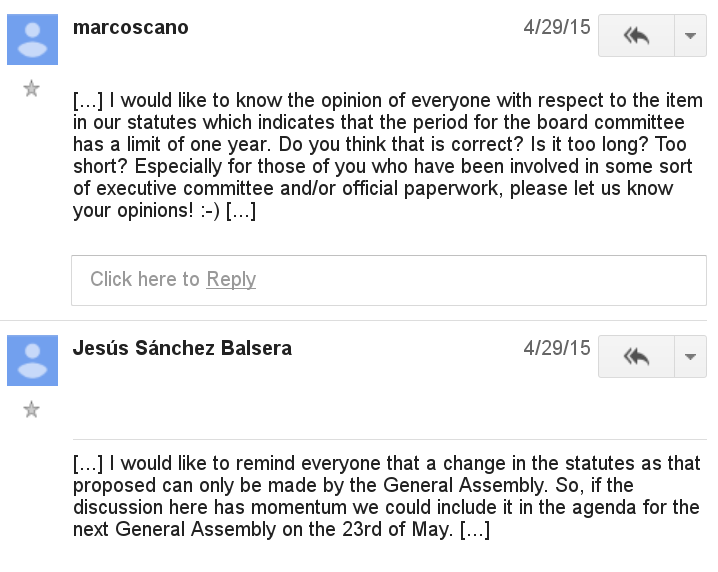
\includegraphics[scale=0.45]{img/quotes_replacement/aed_quote_rules.png}
\caption[Excerpt from a discussion in the mailing list of the members of the Spanish Drupal Association]{Excerpt from a discussion in the public mailing list of the members of the Spanish Drupal Association, original in Spanish. Retrieved \nth{6} May 2016, from \url{https://groups.google.com/forum/\#!topic/asociacion-espanola-de-drupal/4CAtOPsYAVU}.}
\label{quote_aed}
\end{figure}

Another example of the increase in formalisation affecting the rules relates to that regarding the election of committee members. As illustrated by the previous excerpt by I\textunderscript{5}, the initial informal meeting in which positions were elected by the six Drupalistas present resembles the ``do-ocratic" characteristics of smaller local events. This previous environment operates successfully for the purest forms of ``do-ocracy" in which the number of participants remains small. In contrast, as the community grows, collective choice arrangements and more formal and explicit rules are defined in ways which make them modifiable by those who are affected by them. For example, in this specific case, the election of these members is nowadays carried out by a General Assembly, hence illustrating the creation of more formal structures to decentralise decision-making, which is also reflected in a more formal division of labour. Figure \ref{spanish-drupal-assoc-dol} depicts the organisational chart of a local Drupal institution with more explicit and formal roles --- from left to right: president, treasurer, secretary and board members.

\begin{figure}[H]
\centering
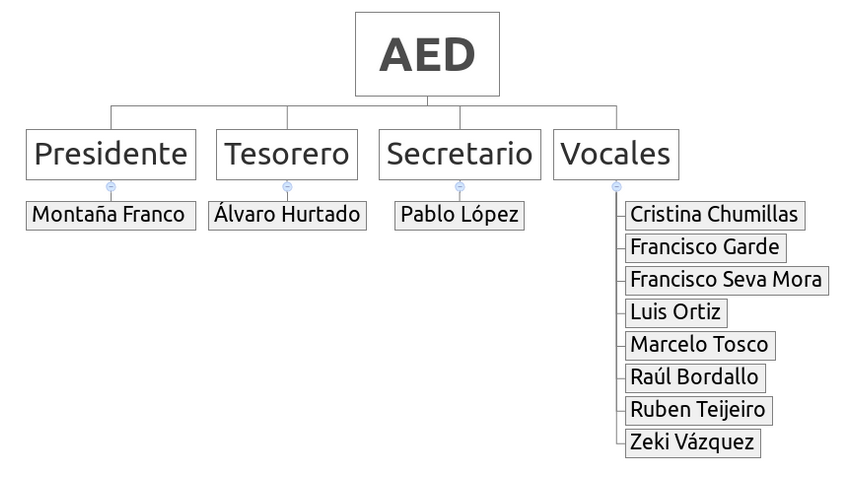
\includegraphics[scale=0.4]{img/offline/aed_organigram}
\caption[Spanish Drupal Association organisational chart]%
{Example of an organisational chart of the Spanish Drupal Association, illustrating a more formal division of labour, including a more formalised set of collective-choice arrangements for decision-making (see \url{http://asociaciondrupal.es/es/grupos-de-trabajo} for further details). Retrieved \nth{13} January 2016, from \url{http://asociaciondrupal.es/es/organigrama-de-la-aed}.}
\label{spanish-drupal-assoc-dol}
\end{figure}

Overall, the general organisational changes experienced over time in this socio-technical system of contribution resemble those previously discussed for the case of ``mostly-online" activities. As the community grows, the informality on which these ``do-ocratic" organisational processes originally relied presents problems for scaling up. In this way, a trend towards formalisation is usually found as a way to increase the legitimacy of decision-making while facilitating its decentralisation over time, as it will also be shown in the next section with regard to quality assurance. Similarly, when comparing the emergence of more formal and autonomous spaces of these socio-technical systems of contribution, both represent a higher degree of centralisation with regards to the way in which the most informal and distributed types are organised. However, this should be understood as a new type of socio-technical system which is also shaped by the dynamics of formalisation and decentralisation over time, and remains more autonomous and decentralised than \textit{DrupalCons}, similarly to \textit{contributed} projects when compared with \textit{core} projects. These similarities can be found, for example, in the ways the organisation of these events typically starts, as illustrated by I\textunderscript{6} in the following quote:

\begin{quotation}
``[...] that's exactly how London started. You know, you just need a few people locally that go: `Ok, this is a good idea', and there's enough people here that would be interested to come along. I think ... you need some local motivated volunteers, you need a location that will draw enough people for the scale of the DrupalCamp that you want to do, and... a bit of hard work and some passion. That would probably do a DrupalCamp."

\begin{flushright}\footnotesize{Project manager, organiser of local events and \textit{DrupalCamps}, M, 10 years.}\end{flushright}
\end{quotation}

Similarly, although the organisation of \textit{DrupalCamps} requires a higher level of coordination and legitimacy in the community than that of local events, they are still more easily reproduced and extended than \textit{DrupalCons}, as in the case of the development of \textit{contributed} projects when compared with \textit{core} projects. The following excerpt by I\textunderscript{11}, exemplifies a common way in which these events are organised for the first time in new places, after attending others:

\begin{quotation}
``[...] I was inspired mostly by DrupalCamp North West, which we went to a couple of times. [...] having been to DrupalCamp North West, and getting more and more involved in the DrupalCon event, then I just thought: `Fuck it, let's do something in the North East'."

\begin{flushright}\footnotesize{Project manager, organiser of local events and \textit{DrupalCamps}, and volunteers' coordinator at several \textit{DrupalCons}, M, 9 years.}\end{flushright}
\end{quotation}

Similarly, a higher degree of coordination is necessary since an excessive fragmentation could be problematic, in comparison with local events, and in a similar way as when comparing \textit{contributed} modules in Drupal.org with \textit{custom} projects not shared on the main collaboration platform. \textit{DrupalCons} were found to play a relevant role to avoid this excessive fragmentation, as expressed by several organisers of events during the participant-observation at \textit{DrupalCon} Amsterdam:

\begin{quotation}
``[...] he explained to me that at the moment there are so many Camps that one of the hardest things is to find dates that don't conflict, although he explained, ironically, that this is of course a good problem to have. [...] Indeed, concretely in the UK, some of the DrupalCamps next year will try to be merged, and several local communities from other regions showed an interest in joining forces instead of organising their own. [...] Another organiser explained to me that in her country there were many DrupalCamps last year. They were thinking of either not organising the one in her region next year, since the past year was not as well-attended as they thought; or running some sort of more specialised event. For instance, focussing on Drupal 8 presentations only."

\begin{flushright}\footnotesize{Full-field notes during attendance to \textit{DrupalCon} Amsterdam (29/09/2014).}\end{flushright}
\end{quotation}

Overall, when compared with the socio-technical system of local events, the socio-technical system of \textit{DrupalCamps} illustrates the definition of clearer community boundaries, defined through more explicit rights to manage resources, for the organisation of the events in this particular case. More formal and local institutions are constituted, whose rules are transformed to facilitate ways in which individuals affected by the collective choice arrangements can participate in them. These rules, as well as the institutions themselves, are flexible and based on local conditions.

In order to show in wider detail how the dynamics of formalisation and decentralisation are intertwined and shape the day-to-day of decision-making for contribution activities in this system, the focus in the next section will be placed on the selection of presentations for \textit{DrupalCamps}. This is with the aim of establishing comparisons with regard to peer-production processes for quality assurance of different socio-technical systems, as seen previously for the case of the projects with regards to quality assurance regarding source code and the projects themselves.

\subsection*{Selection of presentations in \textit{DrupalCamps}}
\label{subsec:dcamps-dtd}

In contrast with other events self-organised by local communities involving presentations, such as those explored in section \ref{subsec:local-events}, the need to cope with a higher amount of proposals than slots to present required these communities to define peer-reviewing processes and mechanisms for quality assurance. A selection of presentations for a \textit{DrupalCamp} will start with an open call for sessions. The ratio of submissions/slots varies largely depending on the \textit{DrupalCamp}. In smaller and newer events it can be very close to 1 (e.g. 0.85 was the lowest found in the data analysed); while in larger and more competitive events it will typically oscillate between 0.4-0.5\footnote{As in the case of the previous use of quantitative data (see footnote \ref{fn-data}) these are employed to have a general estimation, rather than an accurate one. The data has been obtained as part of the participant-observation as a volunteer in the organisation of events, as well as from figures reported by organisers in the interviews and through the documentary analysis.}.

The call for presentations is typically published at least three or four months before the event, using the website designed for that \textit{DrupalCamp} as the main artefact for collaboration. Drupalistas interested in presenting need to prepare and submit a proposal via the \textit{DrupalCamp} site before a deadline. Figure \ref{dcamp-submission-form} provides an example of a typical form for the submission of presentations. The fields vary depending on the \textit{DrupalCamp}, but typically they have at least a title, description, category and level of expertise of the intended audience. The selection of these fields and values is commonly carried out by the core group of organisers of that \textit{DrupalCamp}. For example, the selection of categories may be designed with the aim of attracting as many attendees as possible, by offering diversity in tracks and levels of expertise.

\begin{figure}[H]
\centering
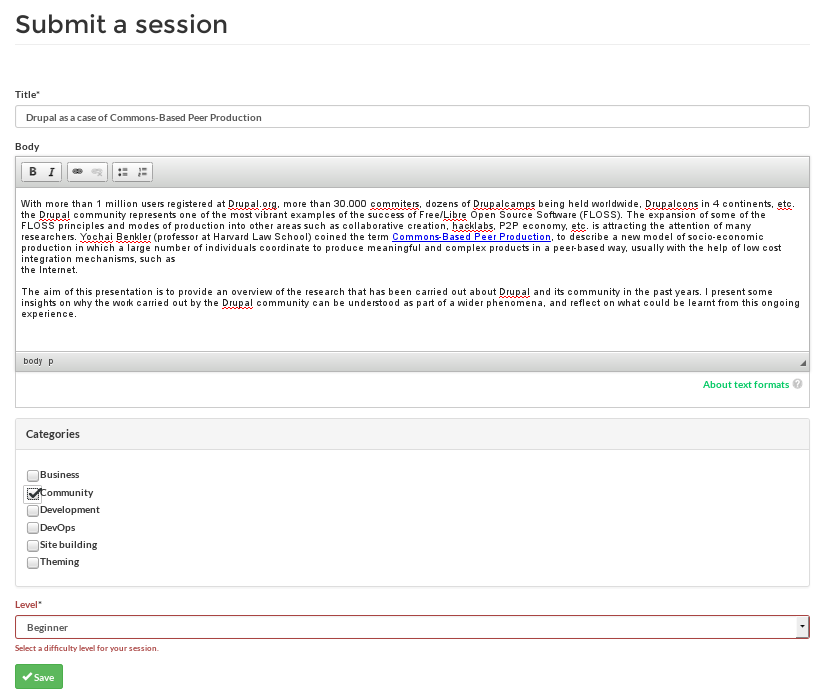
\includegraphics[scale=0.5]{img/offline/call_for_sessions_dcampbrighton}
\caption[Screenshot of the form for a session proposal in \textit{DrupalCamp} Brighton 2016]%
{Screenshot of a form for a session proposal, from \textit{DrupalCamp} Brighton 2016. The set of fields depicted is quite common in most \textit{DrupalCamps}: title, description, categories and level. Retrieved \nth{5} May 2016, from \url{http://www.drupalcampbrighton.co.uk/session/submit}.}
\label{dcamp-submission-form}
\end{figure}

Similarly, the selection criteria of the presentations will typically be decided by the core group of organisers. In most cases, the selection itself will also be carried out by the core group of Drupalistas. The following excerpt by I\textunderscript{6}, exemplifies a typical process for the selection of presentations for a \textit{DrupalCamp}:

\begin{quotation}
``So this is what I was saying a little earlier in comparison, with let's say Drupal Show and Tell [he mentioned before that the selection criteria was not ``very scientific" in that case]. Because it [a DrupalCamp] is a larger scale. [...] Anyone can submit a talk via the website. [...] At that point, we will set a deadline. Once the deadline is hit, we shutdown submissions. We then take those presentations and we try to [...] neutralise them. So, you take away the names, and things like that, so it's less personal. So, you're looking at the description of the talk and the title. That will go into a Google Spreadsheet, and everyone in the core group, let's say about six to seven people can have [a vote] [...] I think there were like 40 talks this year, so we would have 40 votes. And then you just put your ones in those you feel were good. Those were added up between all the people who voted, and then... if you have 0 [votes] , you will not present. If you have 5 or 6 [votes] you will definitely present it... and that was pretty much it, really."

\begin{flushright}\footnotesize{Project manager, organiser of local events and \textit{DrupalCamps}, M, 10 years.}\end{flushright}
\end{quotation}

Several relevant aspects can be extracted from this quote. First of all, the need for a higher degree of monitoring and transparency, related to the higher degree of legitimacy expected, which is argued by the Drupalistas as due to the size of the event, in comparison with local events. As illustrated in this excerpt, as well as in previous sections, the rules in smaller events are typically informal, implicit and the process is carried out by one person. Nevertheless, the organisational processes related to decision-making in these events require a higher degree of legitimacy in the eyes of the community: how is the legitimacy to decide which presentations will be selected obtained in \textit{DrupalCamps}? How can the community ensure that these processes will be fair, avoiding issues such as conflict of interest? This necessity for a higher degree of legitimacy led to a process of formalisation in the mechanisms for decision-making and their rules. For example, in this specific case of the selection of presentations, this produced the emergence of more formal peer-reviewing mechanisms.

The characteristics of these events vary depending on local conditions. For example, the previous quote illustrates how the process encompassed a rudimentary anonymisation of submissions to try to achieve single-blind review properties. In other cases, Drupalistas from other local communities will be invited to carry out the selection to try to minimise possible conflicts of interest. The following excerpt by I\textunderscript{8}, exemplifies a similar process for a \textit{DrupalCamp} in the US, in which anonymisation was employed and external selectors invited to collaborate with local selectors, to try to reduce the possibility of facing conflicts of interest:

\begin{quotation}
``[...] during the selection process, you might guess who could have submitted a session, but you didn't know. And I think one of the strengths of that is... the people who are doing the session selection don't feel pressure to select their friends' talks, or talks from their co-workers. They have a really good excuse when a talk doesn't get selected. They can just go: `Oh, I didn't know'. And they are out of the hook from making up excuses about why something didn't get selected."

\begin{flushright}\footnotesize{Drupal core developer and mentoring organiser, F, 8 years.}\end{flushright}
\end{quotation}

A second relevant aspect with regard to these excerpts concerns the formalisation of the selection criteria. This can be understood under the need to define a set of collective choice agreements which are congruent with the local conditions. It was also observed how, in cases where the events have been running for longer, they also tend to be more formalised and explicitly stated over time. For instance, in the case of \textit{DrupalCamp} Spain, which has been organised over six consecutive years, the collective choice agreements are more explicitly stated when compared to smaller and younger events, also with respect to earlier editions of \textit{DrupalCamp} Spain. This is reflected, for example, in the definition of more specific and detailed sets of guidelines for the topics which are considered more relevant, or for the selection criteria in the call for presentations. They are commonly agreed in internal discussions by the groups of selectors. Indeed, the way in which they are discussed and the final sets of guidelines produced more greatly resemble those of larger events, such as \textit{DrupalCons}, in some cases. This contrasts with the way in which these decisions are made for local events, in which they are typically made by one person and based on implicit social norms, as presented in section \ref{subsec:local-events}. The following extract from the speaker's guidelines from the website of \textit{DrupalCamp} Spain 2016 provides an example of these more formal, explicit speaker guidelines:

\begin{figure}[H]
  \centering
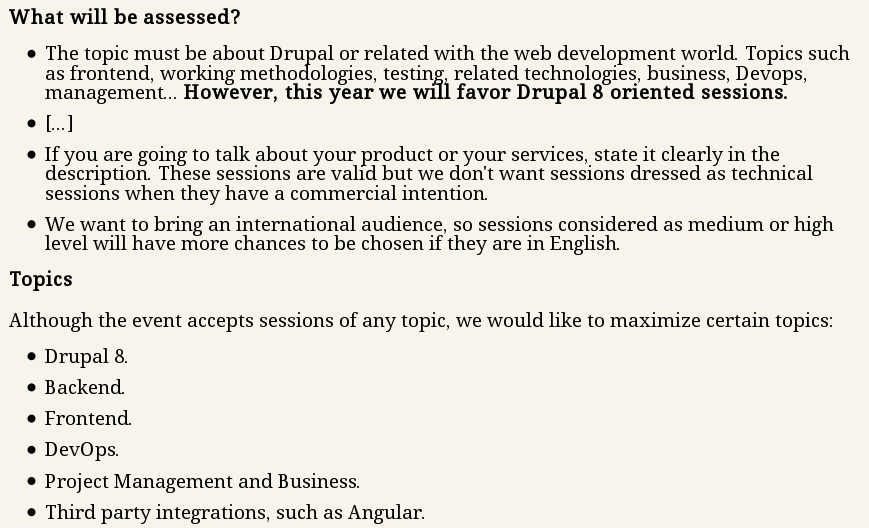
\includegraphics[width=\textwidth]{img/quotes_replacement/speaker_guidelines_dcamp_spain_16.png}
\caption[Excerpt from the speaker guidelines for \textit{DrupalCamp} Spain 2016]{Partial screenshot from speaker guidelines for \textit{DrupalCamp} Spain 2016. Retrieved \nth{5} May 2016, from \url{https://2016.drupalcamp.es/en/content/speaker-guidelines.html}.}
\label{quote_dcamp_guidelines}
\end{figure}

This extract depicts, for example, how talks that potentially promote a company, rather than of general interest for the community, are more likely to be rejected. The goal in this case is similar to the case of quality assurance for presentations at local events --- ``not sales" ---,  however, in the case of \textit{DrupalCamps}, the rules are typically discussed and agreed by the core organisers and they are clearly stated and presentations penalised in the selection, in this case in the form of speaker guidelines: ``we don't want sessions dressed as technical sessions when they have a commercial intention". This is an illustration of how different degrees of formalisation are manifested within the different socio-technical systems that local events and \textit{DrupalCamps} represent.

Overall, the socio-technical system of organisation of \textit{DrupalCamps} possesses a higher degree of formalisation compared to that of local events presented in section \ref{subsec:local-events}. Nevertheless, formalisation remains lower than for the organisation of larger events --- \textit{DrupalCons}. The following excerpts by I\textunderscript{9}, in the context of a conversation about the general organisational processes surrounding the selection of presentations, illustrates how this degree of formalisation is lower for \textit{DrupalCamps} and not even considered formal by some Drupalistas when compared to that of \textit{DrupalCons}, which will be explored in chapter \ref{mostly-offline-cons:chapter}:

\begin{quotation}
``[...] [In DrupalCamps] It's more open, it's not so fixed as a big conference [comparing with DrupalCons]. It's mostly non-profit and community organised [...] So we just build a spreadsheet, and everybody assigns votes, and argues for and against sessions, and then we come to some conclusion. So, I'm not sure if there's a formal process."

\begin{flushright}\footnotesize{Drupal developer and git administrator, M, 8 years.}\end{flushright}
\end{quotation}

Similarly, I\textunderscript{5} compares this degree of formality with respect to that of \textit{DrupalCons}, in the context of a discussion about mechanisms to tackle possible conflicts of interest as those previously aforementioned:

\begin{quotation}
``[...] At DrupalCon there are mechanisms, but I don't think there are these sorts of formal mechanisms established in DrupalCamps, with regards to conflict of interest. Should they exist? Probably. But there aren't so many sessions to select... it's not so formal. But we try. The ideal case would be to find someone who doesn't have any kind of conflict of interest, who doesn't work with any of the session submitters. Who is neither friend nor enemy of them. But that's not possible. And it's not a process that you can open for everyone either [...], because then it would become a popularity contest instead."

\begin{flushright}\footnotesize{Drupal developer and ex-member of the Drupal Association Board of Directors, M, 9 years. Original reply in Spanish.}\end{flushright}
\end{quotation}

In accordance with the organisational processes of \textit{contributed} projects, for the case of ``mostly-online" activities, in this excerpt similar tensions related to the openness to participate in the decision-making can be observed. These socio-technical systems represent intermediate levels with respect to the degree of \textit{organicity}, in which decentralised autonomous spaces for decision-making have emerged. For example, while in the case of the system of \textit{contributed} projects this was reflected in the possibility of participating in the quality assurance and governance of the decision-making of these digital commons; in this case of ``mostly-offline" activities it is reflected in the decision-making for the organisation of the presentations and quality assurance, in this case for the selection of presentations. Similarly, while the legitimacy to carry out this quality assurance originally resides in a de-facto group, an informal network for the case of projects or those local well-known pioneering Drupalistas launching the initiative for the first time, it transited towards a group of maintainers for the case of projects, or towards a more explicit group of reviewers in this case.

In both cases, this has entailed a dynamic of formalisation, in which clearer boundaries with regards to how resources are managed are defined. As in the case of \textit{contributed} projects, the collective choice arrangements vary and are also adapted over time depending on local conditions. For example, the itinerant character of \textit{DrupalCamp} Spain entailed a higher degree of decentralisation via rotation, since the decision-making is carried out by the local community in which the event will be held every year. When the \textit{DrupalCamp} is organised in the same place, as in the case of London, decentralisation was also observed in the decision-making over time, but with a lower level of rotation due to these local conditions. Sporadic volunteers who helped in previous editions and became more involved later were part of these decision-making processes in subsequent editions, while other core organisers decided not to become so involved. Overall, this resembles the transitions presented in section \ref{subsec:contrib-day-by-day} for \textit{contributed} projects. For instance, the trajectory of moving from a regular contributor of patches of a certain \textit{contributed} project, to becoming co-maintainer after being invited by one of the maintainers; or the voluntary rotation of some maintainers after a certain time.

A clearer division of labour can be observed over time, for example in the form of the reviewers, however it is still not as formalised as in the case of \textit{DrupalCons}. As it will be presented in the next chapter, for this socio-technical system of contribution there was also the creation of collective choice agreements for the definition of explicit roles (e.g. track chairs) and the selection of the selectors themselves. This is explained by Drupalistas as dependent on size. For example, I\textunderscript{6} discussed:

\begin{quotation}
``[...] Again... this might be to do with scale. We do have multiple tracks with DrupalCamp London. I think... maybe three or four. But then, if you compare that to a DrupalCon, that's like two or three times. So, we didn't have track chairs or anything like that. So, everyone was voting on all talks, you know? Perhaps... maybe the process doesn't lead the event, the event leads the process."

\begin{flushright}\footnotesize{Project manager, organiser of local events and \textit{DrupalCamps}, M, 10 years.}\end{flushright}
\end{quotation}

Overall, this socio-technical system of contribution can be thought of as a broad set of autonomous spaces for the case of ``mostly-offline" contribution activities, representing a middle layer, in a similar manner as \textit{contributed} projects do in the case of those explored for``mostly-online" contribution activities. Self-organisational processes are more rigid and became more formalised over time, as in the case of \textit{contributed} projects. Similarly, despite the changes in legitimacy for decision-making and the formalisation of responsibilities to maintain and govern these events and the institutions that surround them, there remains a considerable degree of informality in the actions and processes by which they are regulated, when compared with the end of the spectrum: \textit{DrupalCons} for ``mostly-offline" activities, or \textit{core} projects for ``mostly-online" activities.

\section{Conclusion}

Throughout this chapter the study of self-organisational processes of a large and global CBPP community continued, shifting the focus to ``mostly-offline" activities through the exploration of the organisation of events.

Two different socio-technical systems of contribution were explored. Firstly, that composed of local events, characterised for being highly distributed, not requiring a high degree of legitimacy to organise them, and which has scaled up without entailing a higher degree of formalisation over time, but instead remaining more fluid and organic in nature. Secondly, the socio-technical system of \textit{DrupalCamps}, whose self-organisational processes have become more formalised over time, as in the case of \textit{contributed} projects for ``mostly-online" activities.

Similarly to the case of \textit{contributed} projects, this socio-technical system of contribution evolved in a way in which decentralised and local autonomous spaces, in the form of institutions, emerged. Furthermore, it was illustrated how this process of formalisation also responded to the need for a stronger sense of legitimacy, and facilitated the decentralisation of decision-making. While, in the case of \textit{contributed} projects the decentralisation for decision-making pivots around the group of maintainers and co-maintainers of a certain project; whereas in the case of organised events it pivots around the Drupalistas behind the organisation of that specific event and the institutions that surround it. To further understanding on how the dynamics of formalisation and decentralisation operate in this socio-technical system of contribution at a more micro level, the processes of quality assurance were also explored, in this case by studying the selection of presentations. However, it was also discussed how, overall, this system remains more autonomous and organic than that of \textit{DrupalCons}, whose contribution activities represent the most formal type of the ``mostly-offline" activities analysed.

It is precisely to the socio-technical system of \textit{DrupalCons} that the focus will be shifted throughout the next chapter. This is with the aim of concluding the exploration of the general dynamics of formalisation and decentralisation, while allowing comparisons between the different degrees and ways in which the identified dynamics affected the self-organisational processes, despite both systems being focussed on the organisation of events. In addition, this will allow a general analysis considering these different degrees of formalisation for socio-technical systems along the ``mostly-online/mostly-offline" spectrum of contribution activities.